\chapter{Diffraction of a Gaussian probe beam}
\label{app:GaussianBeamDiffraction}


\section{Kirchhoff scalar-diffraction theory}
As discussed in the text surrounding
(\ref{eq:InterferometricMethods:electric_field_eigenvector}),
a CO$_2$ probe beam in a tokamak plasma propagates
as a transverse electromagnetic wave with near-constant polarization
(with any small changes to beam polarization being
of little practical interest to the present work).
Thus, it is suitable to pursue a \emph{scalar} theory
of the beam's interaction with the plasma.
Below, Kirchoff's scalar-diffraction theory is summarized.

A monochromatic scalar wave $U(\vect{r}) e^{-i \omega t}$ in vacuum
satisfies the Helmholtz equation
\begin{equation}
  (\nabla^2 + k^2) U = 0,
\end{equation}
where $k = \omega / c$.
The Helmholtz-Kirchhoff integral theorem states
that the field at a point $P$ is
\begin{equation}
  U(P)
  =
  \frac{1}{4 \pi}
  \int_S \left[
    U \frac{\partial}{\partial n}\left(\frac{e^{i k s}}{s}\right)
    -
    \frac{e^{i k s}}{s} \frac{\partial U}{\partial n}
  \right] dS,
  \label{eq:GaussianBeamDiffraction:Helmholtz_Kirchhoff_integral_theorem}
\end{equation}
where $S$ is an arbitrary surface that encloses $P$,
$\vect{s}$ is the vector from point $P$ to differential area element $dS$,
$\vect{n}$ is the \emph{inward}-pointing normal of surface $S$, and
$U$ is assumed to be differentiable to second order within and on $S$
\cite[Sec.~8.3]{born_and_wolf}.
The relevant geometry is sketched
in Fig.~\ref{fig:GaussianBeamDiffraction:Kirchhoff_geometry}(a).

\begin{figure}
  \centering
  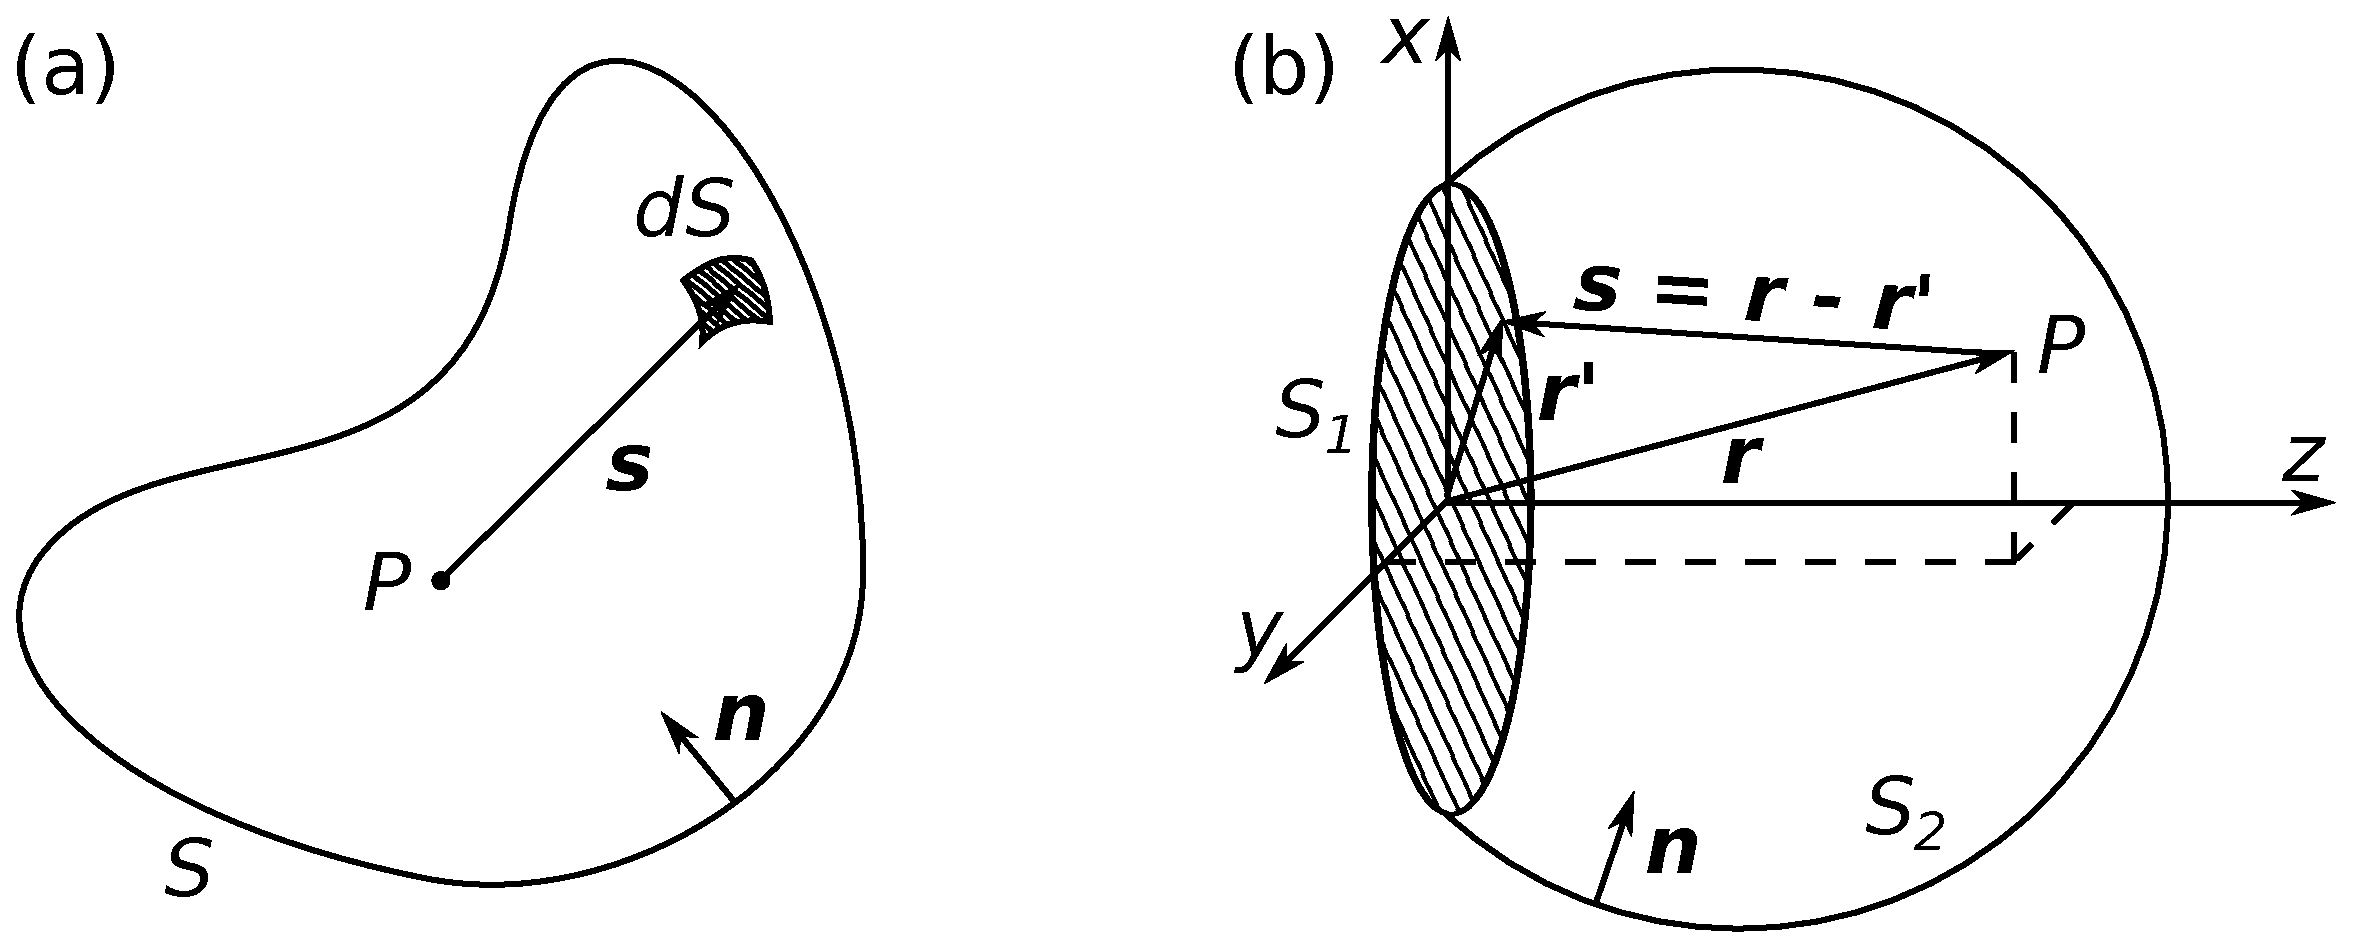
\includegraphics[width = \textwidth]{%
    Appendices/GaussianBeamDiffraction/figs/kirchhoff_geometry.eps}
  \caption[Geometries for Kirchhoff diffraction calculations]{%
    Geometries for Kirchhoff scalar-diffraction calculations.
    When $S_1$ is imaged by an optical system,
    $S_1$ is referred to as the \emph{object plane}.}
\label{fig:GaussianBeamDiffraction:Kirchhoff_geometry}
\end{figure}

To proceed with the diffraction calculation,
assume that the incident waves propagate in the $+z$-direction and
adopt the surface drawn
in Fig.~\ref{fig:GaussianBeamDiffraction:Kirchhoff_geometry}(b).
That is, $S = S_1 + S_2$,
where $S_1$ is a circle in the $(x, y)$-plane, and
$S_2$ is a spherical segment centered on the optical axis.
When $S_1$ is imaged by an optical system,
$S_1$ is referred to as the \emph{object plane}.
Now, assume that the incident waves were ``turned on''
at some finite time in the past, and
take the radius of $S_2$ to be large enough such that
none of the diffracted waves have had sufficient time to reach $S_2$,
i.e.\ $U \equiv 0$ on $S_2$.
(Of course, strictly speaking, the source's finite turn-on time
requires relaxation of the monochromatic assumption.
Finite turn-on time does not preclude a pseudo-monochromatic source, however,
and such a source is assumed hereafter).
Thus, the integral over $S_2$ vanishes, and
the diffraction calculation reduces to an integral over $S_1$.

Now, evaluation of
the Helmholtz-Kirchhoff integral
(\ref{eq:GaussianBeamDiffraction:Helmholtz_Kirchhoff_integral_theorem})
requires knowledge of $U$ on $S_1$.
For free-space propagation,
$S_1$ is an imagined (rather than a physical) surface
that does not impede the propagation of the incident wave $U^{(i)}$
(that is, $U = U^{(i)}$ and
$\partial U / \partial n = \partial U^{(i)} / \partial n$ on $S_1$).
If, however, $S_1$ contains opaque obstacles,
the free-space propagation conditions are no longer valid;
instead, the Kirchhoff boundary conditions can be adopted:
\begin{align}
  \text{surfaces of clear aperture:}&
  \quad
  U = U^{(i)},
  \quad
  \frac{\partial U}{\partial n} = \frac{\partial U^{(i)}}{\partial n},
  \notag \\
  \text{opaque surfaces:}&
  \quad \;
  U = 0,
  \qquad
  \frac{\partial U}{\partial n} = 0.
  \notag
\end{align}
While these boundary conditions are adequate for the current application,
it should be noted that they are not physical
for points that are very close to the boundaries of the opaque obstacles.


\section{Free-space diffraction of a Gaussian beam}
This section demonstrates that the Fraunhofer diffraction formalism
gives the correct form for a free-space Gaussian beam in the far-field limit,
and it also lays the groundwork for examining
the diffraction of a Gaussian beam from plasma-density fluctuations.
Note that the Gaussian-beam definition provided in
Section~\ref{sec:InterferometricMethods:Gaussian_beam_diffraction:Gaussian_beam_definition}
is used throughout the remainder of this appendix.

Assume that the incident Gaussian beam has a waist at $S_1$, and
take the radius of $S_1$ to be much larger than the beam waist $w_0$
such that the domain of integration effectively extends
over the whole $(x, y)$-plane.
For free-space propagation,
$S_1$ does not perturb the Gaussian beam; thus,
$E(\vect{r}, t) = E^{(i)}(\vect{r}, t) = E_G(\vect{r}) e^{-i \omega_0 t}$,
where $E_G(\vect{r})$ is the Gaussian beam's spatial dependence,
as defined by (\ref{eq:InterferometricMethods:Gaussian_beam}).
Now, in the far-field ($k_0 s \gg 1$) and
paraxial ($\vect{s} \approx -z \hat{\vect{z}}$) approximations
\begin{align}
  \left. \frac{e^{i k_0 s}}{s} \right|_{S_1}
  &\approx
  \frac{e^{i k_0 s}}{z},
  \notag \\
  \left. \frac{\partial}{\partial n}
  \left( \frac{e^{i k_0 s}}{s} \right) \right|_{S_1}
  &\approx
  -i k_0 \left( \frac{e^{i k_0 s}}{z} \right).
  \notag
\end{align}
The $s$-dependence in the phase arguments has been retained,
as it is the mechanism responsible for diffraction, but
the $s$-dependence in the amplitude has been dropped
as it only gives rise to negligible variations
in the amplitude of the diffracted wave.
Relative to a spherical wave,
a Gaussian beam has several additional $z$-dependencies;
however, at the beam's waist
\begin{align}
  \left. \frac{\partial w(z)}{\partial z} \right|_{\text{waist}}
  &\equiv
  0,
  \notag \\
  \left. \frac{\partial}{\partial z}
  \left[ \frac{1}{R(z)} \right] \right|_{\text{waist}}
  &=
  \frac{1}{z_R^2},
  \notag \\
  \left. \frac{\partial \psi(z)}{\partial z} \right|_{\text{waist}}
  &=
  \frac{1}{z_R}.
  \notag
\end{align}
Then, if the beam's Rayleigh range is much greater than
the probe wavelength ($k_0 z_R \gg 1$) and
the relevant transverse dimensions are much less than
the Rayleigh range ($w_0 \ll z_R$),
the Gaussian beam at $S_1$ satisfies
\begin{align}
  \left. E_G(\vect{r}') \right|_{S_1}
  &\approx
  E_0 e^{-(\rho' / w_0)^2},
  \notag \\
  \left. \frac{\partial E_G(\vect{r}')}{\partial n} \right|_{S_1}
  &\approx
  i k_0 \left[ E_0 e^{-(\rho' / w_0)^2} \right].
  \notag
\end{align}
Note that the CO$_2$ laser beams ($k_0 \approx \SI{2 \pi e5}{\per\meter}$)
that probe tokamak plasmas often have $z_R \gg \SI{10}{\meter}$
such that $k_0 z_R \gg 1$ and $w_0 \ll z_R$
(the transverse dimensions are constrained by the machine size
such that $w_0 \ll \SI{1}{\meter}$) are very well-satisfied.

Substituting the above expressions for
the incident waves and their surface-normal derivatives into
the Helmholtz-Kirchhoff integral
(\ref{eq:GaussianBeamDiffraction:Helmholtz_Kirchhoff_integral_theorem})
and simplifying yields
\begin{equation}
  E(\vect{r})
  \approx
  \frac{-i E_0}{\lambda_0 z}
  \int_{S_1}
  e^{-( \rho' / w_0 )^2}
  e^{i k_0 s}
  dS.
  \label{eq:GaussianBeamDiffraction:Kirchhoff_diffraction_integral}
\end{equation}
To proceed further, $s$ must be approximated:
\begin{align}
  s
  &=
  | \vect{\rho}' - \vect{r}|
  \notag \\
  &=
  \left[ r^2 - 2(x'x + y'y) + (x'^2 + y'^2) \right]^{1/2}
  \notag \\
  &\approx
  r - \frac{x'x + y'y}{r},
  \label{eq:GaussianBeamDiffraction:Fraunhofer_s}
\end{align}
where only terms linear in $(x' / r)$ and $(y' / r)$ have been retained.
This is known as the Fraunhofer limit, and
it is valid in the far-field $z \gg z_R$~\cite[Sec.~8.3.3]{born_and_wolf}.
Under the Fraunhofer limit
the diffraction integral
(\ref{eq:GaussianBeamDiffraction:Kirchhoff_diffraction_integral}) becomes
\begin{equation}
  E(\vect{r})
  \approx
  \frac{-i E_0}{\lambda_0 z}
  e^{i k_0 r}
  D_x D_y,
  \label{eq:GaussianBeamDiffraction:Fraunhofer_diffracted_field}
\end{equation}
where
\begin{align}
  D_x
  &=
  \int_{-\infty}^{\infty}
  e^{-( x' / w_0 )^2}
  e^{-i k_0 x' x / r}
  dx'
  \label{eq:GaussianBeamDiffraction:Fraunhofer_diffraction_integral_free_space}
  \\
  &=
  \mathcal{F} \left[%
    e^{-( x' / w_0 )^2}
  \right](k_0 x / r)
  \notag \\
  &=
  \sqrt{\pi} w_0 e^{-(k_0 w_0 x / 2 r)^2}
  \label{eq:GaussianBeamDiffraction:Fourier_transform_free_space_Gaussian}
\end{align}
gives the diffraction pattern in the $x$-direction, and
the integral has been easily evaluated by noting that
it is simply the Fourier transform of a Gaussian.
The diffraction pattern in the $y$-direction, $D_y$, is similarly determined.
Note that the $e^{-i k_0 x' x / r} = e^{-i k_0 x' \sin\theta}$ term in
(\ref{eq:GaussianBeamDiffraction:Fraunhofer_diffraction_integral_free_space})
is the typical geometric phase factor
that results from path-length differences between
points on surface $S_1$ and the field point $\vect{r}$, as shown in
Fig.~{\ref{fig:GaussianBeamDiffraction:Fraunhofer_geometric_phase_factor}}.
Substituting
(\ref{eq:GaussianBeamDiffraction:Fourier_transform_free_space_Gaussian}) into
(\ref{eq:GaussianBeamDiffraction:Fraunhofer_diffracted_field}) yields
\begin{equation}
  E(\vect{r})
  \approx
  -i E_0
  \left( \frac{z_R}{z} \right)
  e^{-(k_0 w_0 \rho / 2 r)^2}
  e^{i k_0 r}.
  \label{eq:GaussianBeamDiffraction:Fraunhofer_Gaussian_beam_diffraction}
\end{equation}
Is this consistent
with the expected far-field representation of a Gaussian beam? Yes!
To see this, note that in the far-field ($z \gg z_R$)
\begin{align}
  \frac{z_R}{z}
  &\approx
  \frac{w_0}{w(z)},
  \notag \\
  \frac{k_0 w_0 \rho}{2 r}
  &\approx
  \frac{\rho}{w(z)},
  \notag \\
  r
  &\approx
  z + \frac{\rho^2}{2 R(z)},
  \notag \\
  -i
  = e^{-i \pi / 2}
  &\approx
  e^{-i \psi(z)},
  \notag
\end{align}
such that the diffracted field in the Fraunhofer limit
(\ref{eq:GaussianBeamDiffraction:Fraunhofer_Gaussian_beam_diffraction})
can be cast in the form of a typical Gaussian beam
as expressed in
(\ref{eq:InterferometricMethods:Gaussian_beam}),
i.e.\ $E(\vect{r}) = E_G(\vect{r})$ for $z \gg z_R$.
Of course, when considering free-space propagation,
$E(\vect{r}) \equiv E_G(\vect{r})$ for $0 \leq z < \infty$, but
the above work \emph{proves} that
the Fraunhofer diffraction formalism
gives the correct results under the appropriate limits;
it also lays the groundwork for examining
the diffraction of a phase-modulated Gaussian beam.

\begin{figure}
  \centering
  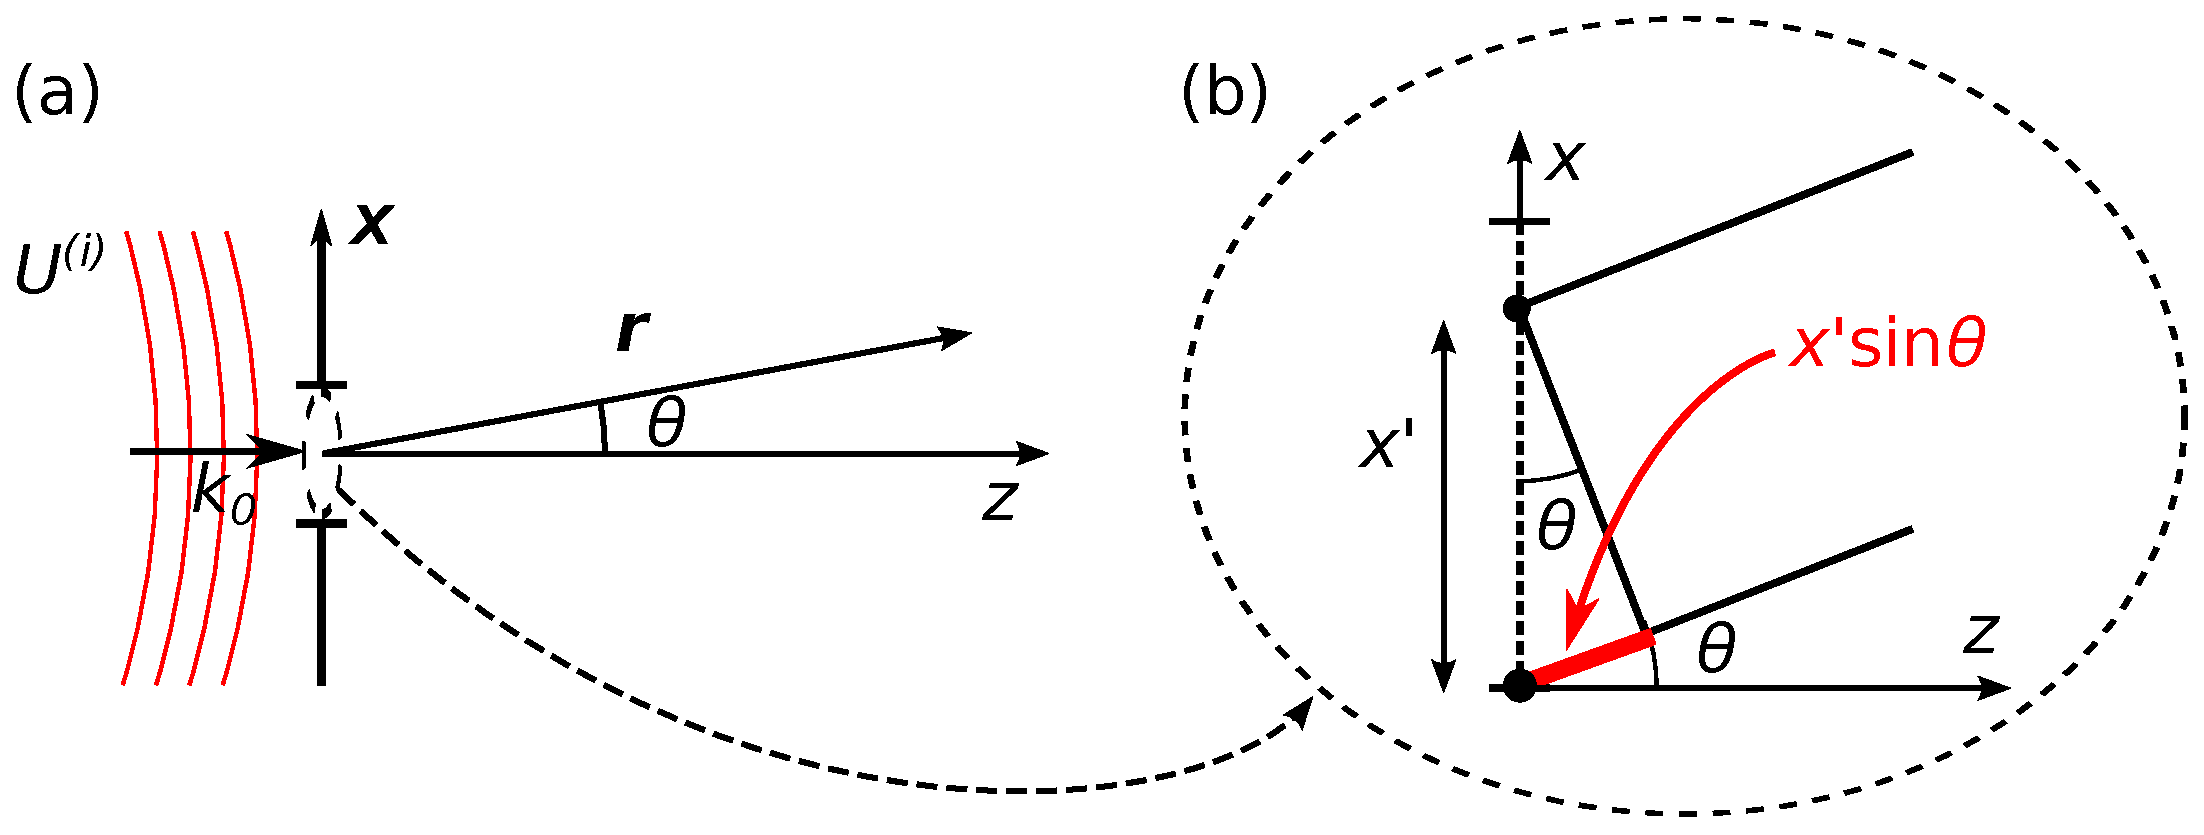
\includegraphics[width = \textwidth]{%
    Appendices/GaussianBeamDiffraction/figs/Fraunhofer_geometric_phase_factor.eps}
  \caption[Fraunhofer geometric phase factor]{%
    (a) Typical Fraunhofer diffraction geometry and
    (b) a close up that displays the path-length difference $x' \sin\theta$
    between a wave emanating from the origin and
    a wave emanating from $x'$}
\label{fig:GaussianBeamDiffraction:Fraunhofer_geometric_phase_factor}
\end{figure}


\section{Diffraction from plasma-density fluctuations}
\label{sec:GaussianBeamDiffraction:from_plasma_density_fluctuations}
Now, allow a Gaussian, CO$_2$ probe beam
to pass through a tokamak plasma.
The beam acquires the plasma-induced phase delay $\phi(\vect{\rho}', t)$
given by (\ref{eq:InterferometricMethods:phase}),
where $\vect{\rho}'$ corresponds to the beam's transverse dimensions.
Explicitly dividing $\phi$ into bulk $\bar{\phi}(t)$ and
spatially varying $\tilde{\phi}(\vect{\rho}', t)$ components,
the plasma-induced phase delay becomes
\begin{equation}
  \phi(\vect{\rho}', t) = \bar{\phi}(t) + \tilde{\phi}(\vect{\rho}', t).
\end{equation}
Typically, $\tilde{\phi}$ varies on much faster time scales than $\bar{\phi}$,
but this is not required.
The spatial variation of the plasma-induced phase delay
contributes to the diffraction of the incident Gaussian probe beam, and
the remainder of this section uses scalar-diffraction theory
to determine the diffracted field in the Fraunhofer limit;
the near-field form consistent with the computed Fraunhofer field
is then inferred.
(The object planes of the imaging systems relevant to this work
sit in the near field, so computation of the imaged field requires
knowledge of the near-field diffraction pattern).

The response functions of the diagnostics investigated in
Sections~\ref{sec:InterferometricMethods:interferometry} and
\ref{sec:InterferometricMethods:pci} are shown
to be linear in their regimes of relevance, so
it is sufficient to examine phase fluctuations $\tilde{\phi}$
consisting of a single Fourier mode
\begin{equation}
  \tilde{\phi}(\vect{\rho}', t) = \tilde{\phi}_0 \cos(k x' - \omega t).
  \label{eq:GaussianBeamDiffraction:cosine_phase_fluctuation}
\end{equation}
As a CO$_2$ beam's optical cycles
($\omega_0 = 2 \pi \cdot \SI{28.3}{\tera\hertz}$)
occur much more rapidly than the temporal evolution of the plasma
($\omega \lesssim 2 \pi \cdot \SI{1}{\giga\hertz}$),
the problem can be treated adiabatically
by solving for the beam propagation
at each instant in time during the relatively slow evolution of $\phi$.
Then, following the formalism pioneered by Raman and Nath
\cite{raman_nath_diffraction_partI,raman_nath_diffraction_partIII},
this plasma-induced phase delay makes an additional phase contribution
to the diffraction integral
(\ref{eq:GaussianBeamDiffraction:Fraunhofer_diffraction_integral_free_space})
such that the diffraction pattern in the $x$-direction is given as
\begin{align}
  D_x
  &=
  \int_{-\infty}^{\infty}
  e^{-( x' / w_0 )^2}
  e^{-i k_0 x x' / r}
  e^{i \phi(x', t)}
  dx'
  \notag \\
  &=
  e^{i \bar{\phi}}
  \int_{-\infty}^{\infty}
  e^{-( x' / w_0 )^2}
  e^{-i k_0 x x' / r}
  e^{i \tilde{\phi}_0 \cos(k x' - \omega t)}
  dx'
  \notag \\
  &\begin{aligned}
    =
    e^{i \bar{\phi}}
    &\int_{-\infty}^{\infty}
    e^{-( x' / w_0 )^2}
    e^{-i k_0 x x' / r}
    \\
    &\times
    \left\{%
      \sum_{m = -\infty}^{\infty}
      i^m \left[ J_m(\tilde{\phi}_0) \right]
      e^{i m (k x' - \omega t)}
    \right\}
    dx'
  \end{aligned}
  \notag \\
  &\begin{aligned}
    =
    e^{i \bar{\phi}}
    &\sum_{m = -\infty}^{\infty}
    i^m \left[ J_m(\tilde{\phi}_0) \right]
    e^{-i m \omega t}
    \\
    &\times
    \int_{-\infty}^{\infty}
    e^{-( x' / w_0 )^2}
    e^{-i \left( \frac{k_0 x}{r} - m k \right) x'}
    dx'
  \end{aligned}
  \notag \\
  &\begin{aligned}
    =
    \sqrt{\pi} w_0
    e^{i \bar{\phi}}
    \sum_{m = -\infty}^{\infty}
    \biggl\{
      &i^m \left[ J_m(\tilde{\phi}_0) \right]
      e^{-i m \omega t}
      \\
      &\qquad \times
      e^{-\left[ \frac{w_0}{2} \left( \frac{k_0 x}{r} - m k \right) \right]^2}
    \biggr\},
  \end{aligned}
  \label{eq:GaussianBeamDiffraction:Fraunhofer_diffraction_integral_phase_modulated}
\end{align}
where the bracketed expression in the third equality follows from
application of the well-known Jacobi-Anger expansion and
$J_m$ is the $m$\ts{th} Bessel function of the first kind.
Noting that $E(\vect{r}, t) = E(\vect{r}) e^{-i \omega_0 t}$,
substitution of
(\ref{eq:GaussianBeamDiffraction:Fraunhofer_diffraction_integral_phase_modulated})
into (\ref{eq:GaussianBeamDiffraction:Fraunhofer_diffracted_field}) yields
\begin{align}
  \begin{aligned}
    E(\vect{r}, t)
    \approx
    &\sum_{m = -1}^{1}
    i^m \left[ J_m(\tilde{\phi}_0) \right]
    e^{-i m \omega t}
    e^{-\left[ \frac{w_0}{2} \left( \frac{k_0 x}{r} - m k \right) \right]^2}
    \\
    &\times
    e^{i \bar{\phi}}
    \left[
      -i E_0
      \left( \frac{z_R}{z} \right)
      e^{-(k_0 w_0 y / 2 r)^2}
      e^{i (k_0 r - \omega_0 t)}
    \right].
  \label{eq:GaussianBeamDiffraction:Fraunhofer_phase_modulated_Gaussian_beam_diffraction}
  \end{aligned}
\end{align}
Here, only the $|m| \leq 1$ terms have been retained because
$|J_m(\tilde{\phi}_0)| \sim \tilde{\phi}_0^{|m|}$
for experimentally relevant values of $\tilde{\phi}_0 \ll 1$.
(The complete small-argument, asymptotic form for $J_m$ is discussed in
Section~\ref{sec:InterferometricMethods:imaging:weak_coupling_limit}).
The effect of higher order terms can be easily investigated
by e.g.\ including the $m = \pm 2$ terms etc.

\begin{figure}
  \centering
  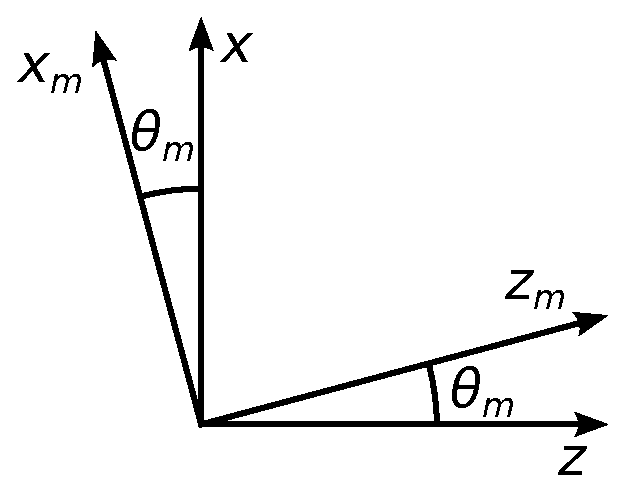
\includegraphics[width = 0.4 \textwidth]{%
    Appendices/GaussianBeamDiffraction/figs/coordinate_rotation.eps}
  \caption{Coordinate transformation for interpretation of
    the diffraction pattern of a phase-modulated Gaussian beam}
\label{fig:GaussianBeamDiffraction:coordinate_rotation}
\end{figure}

To put
(\ref{eq:GaussianBeamDiffraction:Fraunhofer_phase_modulated_Gaussian_beam_diffraction})
in a more familiar form,
consider the coordinate transformation
from the lab-frame coordinate system $\vect{r}$
to the coordinate system of the $m$\ts{th} scattered beam $\vect{r}_m$,
as depicted graphically
in Fig.~\ref{fig:GaussianBeamDiffraction:coordinate_rotation}.
As the transformation is simply
a rotation about the $y$-axis by angle $\theta_m$,
the coordinate systems are related via
\begin{equation}
  \begin{pmatrix}
    x_m
    \\
    y_m
    \\
    z_m
  \end{pmatrix}
  =
  \begin{pmatrix}
    \cos\theta_m & 0 & -\sin\theta_m
    \\
    0            & 1 & 0
    \\
    \sin\theta_m & 0 & \cos\theta_m
  \end{pmatrix}
  \begin{pmatrix}
    x
    \\
    y
    \\
    z
  \end{pmatrix},
  \label{eq:GaussianBeamDiffraction:object_plane_coordinate_transformation_explicit}
\end{equation}
where
\begin{equation}
  \sin \theta_m
  \equiv
  \frac{m k}{k_0}.
  \label{eq:GaussianBeamDiffraction:scattering_angles}
\end{equation}
Typically, $m k / k_0 \ll 1$ such that
\begin{equation}
  \cos \theta_m
  \approx
  1 - \frac{1}{2} \left( \frac{m k}{k_0} \right)^2
\end{equation}
is a very good approximation.
The above coordinate transformation can be written more compactly as
\begin{equation}
  \vect{r}_m
  =
  [ \vect{R}(\theta_m) ] \vect{r},
  \label{eq:GaussianBeamDiffraction:object_plane_coordinate_transformation_compact}
\end{equation}
where
\begin{equation}
  \vect{R}(\theta)
  =
  \begin{pmatrix}
    \cos\theta & 0 & -\sin\theta
    \\
    0          & 1 & 0
    \\
    \sin\theta & 0 & \cos\theta
  \end{pmatrix}
  \label{eq:GaussianBeamDiffraction:rotation_matrix}
\end{equation}
is the rotation matrix
that rotates the $(x, z)$-plane about the $y$-axis by angle $\theta$.
Rotation matrices are \emph{orthogonal},
which endows $\vect{R}(\theta_m)$ with some useful properties
\cite[Ch.~6]{FB_linear_algebra};
namely, its inverse is equal to its transpose $[\vect{R}(\theta_m)]^T$
\begin{equation}
  [\vect{R}(\theta_m)]^T
  =
  [\vect{R}(\theta_m)]^{-1}
  =
  \vect{R}(-\theta_m),
  \label{eq:GaussianBeamDiffraction:rotation_matrix_inverse_relationships}
\end{equation}
and its determinant is unity
\begin{equation}
  \text{det}[\vect{R}(\theta_m)] = |\vect{R}(\theta_m)| = 1
  \label{eq:GaussianBeamDiffraction:rotation_matrix_determinant}
\end{equation}
such that the rotation preserves lengths, i.e.\ $r_m = r$.
It is sufficient to retain terms only to first order in
$k / k_0$ (small scattering angle) and $x / z$ (paraxial limit)
for the \emph{amplitude} dependencies of the diffracted field
(this is \emph{not}, in general, true for the phase dependencies).
Thus, $1 / z \approx 1 / z_m$ and $x \approx x_m + (m k / k_0) z$
such that the Fraunhofer diffracted field
(\ref{eq:GaussianBeamDiffraction:Fraunhofer_phase_modulated_Gaussian_beam_diffraction})
can be rewritten as
\begin{equation}
  \begin{aligned}
    E(\vect{r}, t)
    \approx
    e^{i \bar{\phi}}
    &\sum_{m = -1}^{1}
    i^m \left[ J_m(\tilde{\phi}_0) \right]
    e^{-i (\omega_0 + m \omega) t}
    \\
    &\times
    \left[
      -i E_0
      \left( \frac{z_R}{z_m} \right)
      e^{-(k_0 w_0 \rho_m / 2 r)^2}
      e^{i k_0 r}
    \right],
  \end{aligned}
\end{equation}
where $\rho_m = (x_m^2 + y_m^2)^{1/2}$.
Now, the bracketed expression has the form of
(\ref{eq:GaussianBeamDiffraction:Fraunhofer_Gaussian_beam_diffraction})
for a far-field Gaussian beam; thus,
the diffracted electric field can be more compactly and generally written as
\begin{equation}
  E(\vect{r}, t)
  \approx
  e^{i \bar{\phi}}
  \sum_{m = -1}^{1}
  i^m \left[ J_m(\tilde{\phi}_0) \right]
  E_G(\vect{r}_m)
  e^{-i (\omega_0 + m \omega) t}.
  \label{eq:GaussianBeamDiffraction:phase_modulated_Gaussian_beam_diffraction}
\end{equation}
Note that
(\ref{eq:GaussianBeamDiffraction:phase_modulated_Gaussian_beam_diffraction})
is valid for $0 \leq z < \infty$ rather than only for $z \gg z_R$;
that is, computing the far-field diffraction pattern
has additionally allowed \emph{inferring} the corresponding near field.

Thus, a sinusoidal phase modulation diffracts an incident Gaussian beam
predominantly into downscattered ($m = -1$), unscattered ($m = 0$), and
upscattered ($m = 1$) Gaussian beams.
The incident beam is coupled into the $m$\ts{th} scattered beam
with strength $J_m(\tilde{\phi}_0)$.
The $m$\ts{th} scattered beam is Doppler shifted
relative to the incident beam by $m \omega$ and
propagates at an angle $\theta_m \approx m k / k_0$
relative to the lab-frame optical axis.
The adiabatic assumption ($\omega / \omega_0 \ll 1$)
is very well-satisfied for a CO$_2$ probe beam
in a typical tokamak plasma
(i.e.\
$\omega / \omega_0
\lesssim
\SI{1}{\giga\hertz} / \SI{28.3}{\tera\hertz}
\sim 10^{-5}$).
Thus, the scattering is very nearly elastic, and
$|\vect{k}_{0,m}| = k_0$ is a very good approximation.
This constraint of elasticity
coupled with knowledge of the scattering angle $\theta_m$
allows determination of the scattered wavevector
\begin{equation}
  \vect{k}_{0,m}
  =
  (m k) \hat{\vect{x}}
  +
  k_0 \left[ 1 - \left(\frac{m k}{k_0}\right)^2 \right]^{1/2} \hat{\vect{z}}.
  %k_0 \sqrt{1 - \left(\frac{m k}{k_0}\right)^2} \hat{\vect{z}}
  \label{eq:GaussianBeamDiffraction:scattered_beam_wavevector}
\end{equation}
Finally, note that the simultaneous presence
of both the upscattered and downscattered beams
under typical experimental conditions
has been demonstrated empirically
\cite[Sec.~2.1]{dorris_phd}.
In the above formalism, the simultaneous upscattering and downscattering
of the incident probe beam results from
the assumption of a sinusoidal phase fluctuation in
(\ref{eq:GaussianBeamDiffraction:cosine_phase_fluctuation});
if a complex exponential were assumed instead,
one would erroneously deduce that
only one such scattering process (either up or down) occurs.


\section{Validity of the Raman-Nath formalism}
The Raman-Nath formalism employed in
Section~\ref{sec:GaussianBeamDiffraction:from_plasma_density_fluctuations}
is valid as long as the fluctuation wavenumber $k$ is not ``too large''.
This constraint has been rigorously quantified by Bhatia and Noble
\cite{bhatia_53_general_theory,bhatia_53_approximate_expressions_for_intensities} and
is also discussed by Born and Wolf
\cite[Ch.~12]{born_and_wolf}.
Specifically, beam diffraction will be in the Raman-Nath regime when
\begin{equation}
  \delta = \frac{\tilde{n}_e}{\bar{n}_e} \left( \frac{k_0}{k} \right)^2 \gg 1,
  \label{eq:GaussianBeamDiffraction:raman_nath_validity_criterion}
\end{equation}
where
$\bar{n}_e$ is the bulk plasma density,
$\tilde{n}_e$ is the amplitude of the plasma-density fluctuation,
$k_0$ is the vacuum wavenumber of the probe beam, and
$k$ is the wavenumber of the plasma-density fluctuation.
Note that the above $\delta$ is equivalent
to that used by Bhatia and Noble,
after having made the appropriate substitutions
for a CO$_2$ probe beam in a tokamak plasma.
Assuming typical tokamak values
\begin{align}
  &\frac{\tilde{n}_e}{\bar{n}_e}
  \sim
  10^{-3},
  \notag \\
  &k
  \lesssim
  \SI{30}{\per\centi\meter}
  \notag
\end{align}
yields $\delta \gtrsim 40$
for a CO$_2$ probe beam ($k_0 \approx 2 \pi \cdot \SI{e5}{\per\meter}$)
such that beam's diffraction is well within the Raman-Nath regime.
In the opposite regime ($\delta \ll 1$)
the beam can \emph{Bragg scatter} from the phase fluctuation,
producing a single, strongly-scattered beam
\cite{bhatia_53_approximate_expressions_for_intensities}
\cite[Ch.~12]{born_and_wolf};
such Bragg scattering is the foundation of acousto-optics.


\section{Wavenumber filtering of the diffracted field}
Examine again the diffracted field
(\ref{eq:GaussianBeamDiffraction:phase_modulated_Gaussian_beam_diffraction}).
The spatial dependence of each term in the summation
is wholly governed by the factor $E_G(\vect{r}_m)$,
which corresponds to a Gaussian beam
that emanates from the beam waist
at an angle $\theta_m$ relative to the lab-frame $z$-axis.
The coordinate system $\vect{r}_m$ is defined such that
the $m$\ts{th} Gaussian beam propagates along the $z_m$-axis, and
it is related to the lab-frame coordinate system $\vect{r}$ via
(\ref{eq:GaussianBeamDiffraction:object_plane_coordinate_transformation_compact}).
The wavenumber basis $\vect{k}_m$ that is dual to $\vect{r}_m$
is similarly related to the lab-frame wavenumber basis $\vect{k}$ via
\begin{equation}
  \vect{k}_m
  =
  [ \vect{R}(\theta_m) ] \vect{k},
  \label{eq:GaussianBeamDiffraction:object_plane_coordinate_transformation_wavenumber_dual}
\end{equation}
which naturally results from the geometric constraint that
$\vect{k} \cdot \vect{r} = \vect{k}_m \cdot \vect{r}_m$.

Imagine now that each of the above Gaussian beams
is somehow manipulated based upon its Fourier wavenumber content.
Assume this manipulation can be described
in terms of a transfer function $T(\vect{k})$,
where $\vect{k}$ is the lab-frame wavenumber basis.
A transfer function of this form is appropriate for investigating e.g.\
diffraction from an aperture or the action of a phase plate.
Using the wavenumber basis transformation
(\ref{eq:GaussianBeamDiffraction:object_plane_coordinate_transformation_wavenumber_dual}),
this transfer function can be written
in terms of the $\vect{k}_m$ wavenumber basis as
\begin{equation}
  T(\vect{k}) = T(\vect{R}_{-m} \vect{k}_m),
\end{equation}
where the abbreviation $\vect{R}_m = \vect{R}(\theta_m)$ has been adopted.
The transformed field $E_T$ then has the Fourier representation
in the $\vect{k}_m$ wavenumber basis
\begin{equation}
  E_T(\vect{k}_m) = T(\vect{R}_{-m} \vect{k}_m) \cdot E_G(\vect{k}_m).
\end{equation}
Inverse Fourier transforming $E_T(\vect{k}_m)$ yields
\begin{equation}
  E_T(\vect{r}_m)
  =
  \frac{1}{(2 \pi)^3}
  \int d\vect{k}_m \,
  \left[%
    T(\vect{R}_{-m} \vect{k}_m)
    e^{i \vect{k}_m \cdot \vect{r}_m}
  \right]
  E_G(\vect{k}_m).
\end{equation}
Note that each spectral component $E_G(\vect{k}_m)$
individually satisfies the wave equation.
Thus, the above construction of the transformed field $E_T(\vect{r}_m)$,
which consists of a linear combination of the spectral components
with arbitrary amplitudes and phases,
\emph{also} satisfies the wave equation.
Now, explicitly writing $E_G(\vect{k}_m)$ as the Fourier transform
of $E_G$ over a dummy spatial coordinate $\vect{r}'$, and
exchanging the order of integration yields
\begin{equation}
  E_T(\vect{r}_m)
  =
  \frac{1}{(2 \pi)^3}
  \int d\vect{r}' \,
  E_G(\vect{r}')
  \int d\vect{k}_m \,
  T(\vect{R}_{-m} \vect{k}_m)
  e^{i \vect{k}_m \cdot (\vect{r}_m - \vect{r}')}.
\end{equation}
Further, for the applications considered here,
it is advantageous to change the variables of integration
from the $\vect{k}_m$ wavenumber basis
to the lab-frame wavenumber basis $\vect{k}$.
Note that
\begin{equation}
  d\vect{k}_m
  =
  \left| \frac{\partial \vect{k}_m}{\partial \vect{k}} \right|
  d\vect{k}
  =
  |\vect{R}_m|
  d\vect{k}
  =
  d\vect{k}
\end{equation}
and that
\begin{align}
  \vect{k}_m \cdot (\vect{r}_m - \vect{r}')
  &=
  (\vect{R}_m \vect{k}) \cdot (\vect{r}_m - \vect{r}')
  \notag \\
  &=
  (\vect{R}_m \vect{k})^T (\vect{r}_m - \vect{r}')
  \notag \\
  &=
  \vect{k}^T \vect{R}_m^T (\vect{r}_m - \vect{r}')
  \notag \\
  &=
  \vect{k} \cdot [\vect{R}_{-m} (\vect{r}_m - \vect{r}')]
\end{align}
such that the transformed field $E_T(\vect{r}_m)$ becomes
\begin{equation}
  E_T(\vect{r}_m)
  =
  \frac{1}{(2 \pi)^3}
  \int d\vect{r}' \,
  E_G(\vect{r}')
  \int d\vect{k} \,
  T(\vect{k})
  e^{i \vect{k} \cdot \left[ \vect{R}_{-m} (\vect{r}_m - \vect{r}') \right]},
  \label{eq:GaussianBeamDiffraction:mth_diffracted_beam_Fourier_filtered}
\end{equation}
where, again, the abbreviation $\vect{R}_{-m} = \vect{R}(-\theta_m)$
has been adopted and $\vect{R}(\theta)$ is the rotation matrix given by
(\ref{eq:GaussianBeamDiffraction:rotation_matrix}).

To make further progress,
a particular form of $T(\vect{k})$ is needed.
Assume that wavenumbers are filtered
only in the direction of beam scattering
i.e.\ $T(\vect{k}) = T(k_x)$.
(For example, the groove of a phase plate would be aligned
with the lab-frame $y$-axis to effect such filtering).
Then
\begin{equation}
  \vect{R}_{-m} (\vect{r}_m - \vect{r}')
  =
  \begin{pmatrix}
    (x_m - x') \cos\theta_m + (z_m - z') \sin\theta_m
    \\
    y_m - y'
    \\
    (z_m - z') \cos\theta_m - (x_m - x') \sin\theta_m
  \end{pmatrix}
\end{equation}
such that
(\ref{eq:GaussianBeamDiffraction:mth_diffracted_beam_Fourier_filtered})
becomes
\begin{align}
  E_T(\vect{r}_m)
  &=
  \frac{1}{(2 \pi)^3}
  \int d\vect{r}' \,
  E_G(\vect{r}')
  \int dk_y \,
  e^{i k_y (y_m - y')}
  \notag \\
  &\qquad\quad \times
  \int dk_z \,
  e^{i k_z [(z_m - z') \cos\theta_m - (x_m - x') \sin\theta_m]}
  \notag \\
  &\qquad\quad \times
  \int dk_x \,
  T(k_x)
  e^{i k_x \left[ (x_m - x') \cos\theta_m + (z_m - z') \sin\theta_m \right]}
  \notag \\
  &=
  \frac{1}{2 \pi}
  \int d\vect{r}' \,
  E_G(\vect{r}')
  \delta(y_m - y')
  \notag \\
  &\qquad\quad \times
  \delta\bigl( (z_m - z') \cos\theta_m - (x_m - x') \sin\theta_m \bigr)
  \notag \\
  &\qquad\quad \times
  \int dk_x \,
  T(k_x)
  e^{i k_x \left[ (x_m - x') \cos\theta_m + (z_m - z') \sin\theta_m \right]}
  \notag \\
  &\begin{aligned}
    &=
    \frac{1}{2 \pi}
    \int dx' \,
    E_G\bigl( x',\, y_m,\, z_m - (x_m - x')\tan \theta_m \bigr)
    \\
    &\qquad\quad \times
    \int dk_x \,
    T(k_x)
    e^{i k_x (x_m - x') \sec\theta_m}
  \end{aligned}
  \label{eq:GaussianBeamDiffraction:mth_diffracted_beam_kx_filtered_v1}
\end{align}
Contributions to the integral from regions outside of $|x'| \lesssim w(z_m)$
are suppressed by the Gaussian envelope such that
\begin{align}
  w\bigl( z_m - (x_m - x')\tan \theta_m \bigr)
  &\approx
  w(z_m),
  \notag \\
  R\bigl( z_m - (x_m - x')\tan \theta_m \bigr)
  &\approx
  R(z_m),
  \notag \\
  \psi\bigl( z_m - (x_m - x')\tan \theta_m \bigr)
  &\approx
  \psi(z_m)
  \notag
\end{align}
are very good approximations.
Note that the phase of the Gaussian beam
\emph{cannot} be approximated in such a manner;
instead, terms up to first order in $\theta_m$
must be retained in the phase.
After making these approximations,
(\ref{eq:GaussianBeamDiffraction:mth_diffracted_beam_kx_filtered_v1})
reduces to
\begin{equation}
  E_T(\vect{r}_m)
  \approx
  E_G(0, y_m, z_m)
  \cdot
  \mathcal{E}(\vect{r}_m, k),
  \label{eq:GaussianBeamDiffraction:mth_diffracted_beam_kx_filtered_compact}
\end{equation}
where
\begin{equation}
  \begin{aligned}
    \mathcal{E}(\vect{r}_m, k)
    &=
    \frac{e^{-i m k x_m}}{2 \pi}
    \\
    &\quad \times
    \int dx' \,
    \exp\left[ \frac{-x'^2}{w(z_m)^2} \right]
    \exp\left\{%
      i \left[%
        m k x'
        +
        \frac{k_0 x'^2}{2 R(z_m)}
      \right]
    \right\}
    \\
    &\quad \times
    \int dk_x \,
    T(k_x)
    e^{i k_x (x_m - x')}
  \end{aligned}
  \label{eq:GaussianBeamDiffraction:mth_diffracted_beam_kx_filtered_transformation}
\end{equation}
is a complex-valued function
that describes the amplitude and phase transformations
that result from filtering the scattered radiation by $T(k_x)$.
(Note that
(\ref{eq:GaussianBeamDiffraction:mth_diffracted_beam_kx_filtered_compact})
readily reduces to $E_T(\vect{r}_m) = E_G(\vect{r}_m)$ when $T(k_x) = 1$,
in agreement with expectations).
Generalizing
(\ref{eq:GaussianBeamDiffraction:phase_modulated_Gaussian_beam_diffraction})
to allow for such wavenumber-dependent manipulation
yields a total diffracted electric field
\begin{equation}
  E(\vect{r}, t)
  \approx
  e^{i \bar{\phi}}
  \sum_{m = -1}^{1}
  i^m \left[ J_m(\tilde{\phi}_0) \right]
  E_T(\vect{r}_m)
  e^{-i (\omega_0 + m \omega) t}.
  \label{eq:GaussianBeamDiffraction:phase_modulated_Gaussian_beam_diffraction_Fourier_filtered}
\end{equation}
Manipulating the total diffracted electric field in such a manner
forms the foundation of phase contrast imaging (PCI),
as is discussed in Section~\ref{sec:InterferometricMethods:pci}.


\bibliographystyle{plainurl}
\bibliography{references}
